\section{Theory}

\subsection{Begriffe und Klassifikation}

\subsubsection{Ordnung}

Wie bei gewöhnlichen Differentialgleichungen ist die Ordnung
die höchste Ableitung der unbekannten Funktion, die in der
Differentialgleichung vorkommt.\\

\textbf{PDGL 1. Ordnung: } \qquad$F\biggl(x_1,\dots,x_n, u, \frac{\partial u}{\partial x_1},\dots,\frac{\partial u}{\partial x_n}\biggr)$

Sie kann durch Substitution $\frac{\partial u}{\partial x_i}\to p_i$ durch  $F(x_1,\dots,x_n,u,p_1,\dots,p_n),$
ausgedrückt werden.\\

\textbf{PDGL 2. Ordnung: } \qquad $F\biggl(x_1,\dots,x_n,u,
\frac{\partial u}{\partial x_1},\dots,\frac{\partial u}{\partial x_n},
\frac{\partial^2 u}{\partial x_1^2},\dots,\frac{\partial^2 u}{\partial x_n^2}\biggr)$

Sie kann durch Substitution $\frac{\partial u}{\partial x_i}\to p_i,~\frac{\partial^2 u}{\partial x_i\partial x_j}\to t_{ij}$ durch
$F(x_1,\dots,x_n,u,p_1,\dots,p_n,t_{11},t_{12},\dots,t_{n,n-1},t_{nn})$
ausgedrückt werden.\\
\textbf{Beispiel Übung}\\
\begin{tabular}{lclcl}
$\frac{\partial^2 u}{\partial x_1 \partial x_2} = 0$ & $\Rightarrow$ & 
    $F(t_{12}) = t_{12} = 0$ & $\Leftrightarrow$ &
    $F \left( \frac {\partial^2 u}{\partial x_1 \partial x_2} \right) = 0$ \\
$\frac{\partial u}{\partial x_1} = \frac{\partial u}{\partial x_2} $ & $\Rightarrow$ & 
    $F(p_1,p_2) = p_1 - p_2 = 0$ & $\Leftrightarrow$ & 
    $F \left( \frac{\partial u}{\partial x_1}, \frac{\partial u}{\partial x_2} \right) = 0$ \\
$x_1 \frac{\partial u}{\partial x_1} + x_2 \frac{\partial u}{\partial x_2} = \frac{\partial u}{\partial x_3} $ & 
    $\Rightarrow$ & $F(x_1,x_2,p_1,p_2,p_3) = x_1 p_1 + x_2 p_2 - p_3$ & $\Leftrightarrow$ &
    $F\left( x_1,x_2,\frac{\partial u}{\partial x_1},\frac{\partial u}{\partial x_2},\frac{\partial u}{\partial x_3} \right)
    = x_1\frac{\partial u}{\partial x_1} + x_2\frac{\partial u}{\partial x_2} - \frac{\partial u}{\partial x_3} = 0$

\end{tabular}

\subsubsection{Laplace-Operator}
\begin{tabular}{ll}
Kartesisch: $\Delta u(x,y,z)=\frac{\partial^2u}{\partial x^2}+\frac{\partial^2u}{\partial y^2}+\frac{\partial^2u}{\partial z^2}$
& Zylinder: $\Delta f ( \rho , \phi , z ) = \frac{1}{\rho} \frac{\partial}{\partial \rho}
\left( \rho\,\frac{\partial f}{\partial \rho} \right) +
\frac{1}{\rho^2}\frac{\partial^2 f}{\partial \phi^2} +
\frac{\partial^2 f}{\partial z^2}$ \\
Polar: $\Delta f(r, \varphi ) =
\frac{1}{r}\frac{\partial f}{\partial r} r \frac{\partial f}{\partial r} + \frac{1}{r^2} \frac{\partial^2 f}{\partial \varphi^2}$
& Kugel: $\Delta f ( r , \vartheta , \phi ) = \frac{1}{\rho^2}\frac{\partial}{\partial \rho} \left(\rho^2 \frac{\partial f}{\partial \rho}\right) + \frac{1}{\rho^2 \sin\theta} \frac{\partial}{\partial \theta} \left(\sin\theta \frac{\partial f}{\partial \theta}\right) + \frac{1}{\rho^2 \sin^2\theta} \frac{\partial^2 f}{\partial \varphi^2}$
\end{tabular}

\subsubsection{Umwandlung in System niedriger Ordnung}

\begin{tabular}{ll}
Gegeben:& $F\biggl(x,y,u,\frac{\partial u}{\partial x},\frac{\partial u}{\partial y},
\frac{\partial^2 u}{\partial x^2},\frac{\partial^2 u}{\partial x\partial y},
\frac{\partial^2u}{\partial y^2}\biggr)=0.$\\[0.2cm]
Substitution: & $p=\frac{\partial u}{\partial x},\qquad q=\frac{\partial u}{\partial y}$\\[0.2cm]
Für zweite Ableitungen: & $\frac{\partial^2 u}{\partial x^2}=\frac{\partial p}{\partial x},\quad \frac{\partial^2 u}{\partial x\partial y}=\frac{\partial p}{\partial y}=\frac{\partial q}{\partial x},\quad\frac{\partial^2 u}{\partial y^2}=\frac{\partial q}{\partial y}$\\[0.2cm]
Gleichungssystem 1.Ordnung& $p=\frac{\partial u}{\partial x},\quad q=\frac{\partial u}{\partial y},\quad\frac{\partial p}{\partial y}=\frac{\partial q}{\partial x}$
\end{tabular}

\subsubsection{Notationen einer PDGL, Gebiet $\Omega$}
\begin{minipage}{4cm}
	\begin{tabular}{ll}
	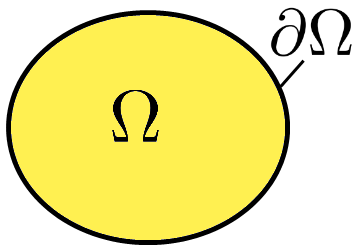
\includegraphics[width=3cm]{Content/01_theory/Gebiet}&
	\end{tabular}
\end{minipage}
\begin{minipage}{4cm}	
	\begin{tabular}{ll}
		$\overset{\circ}{\Omega}$ & Innere Punkte\\
		$\partial\Omega$ & Rand\\
		$\overset{\_}{\Omega}$ & Gebiet $\Omega$ und Rand $\partial\Omega$\\
	\end{tabular}
\end{minipage}

Das Gebiet einer PDGL \textbf{muss} offen sein, nur dann ist die partielle
Ableitung überall definiert. Das Gebiet ist offen, wenn um jeden Punkt im Gebiet
$\Omega$ ein kleiner Ball gezeichnet werden kann, welches sich auch im Gebiet $\Omega$ befindet.\\

\begin{minipage}{4cm}
	Kein Gebiet:\\
	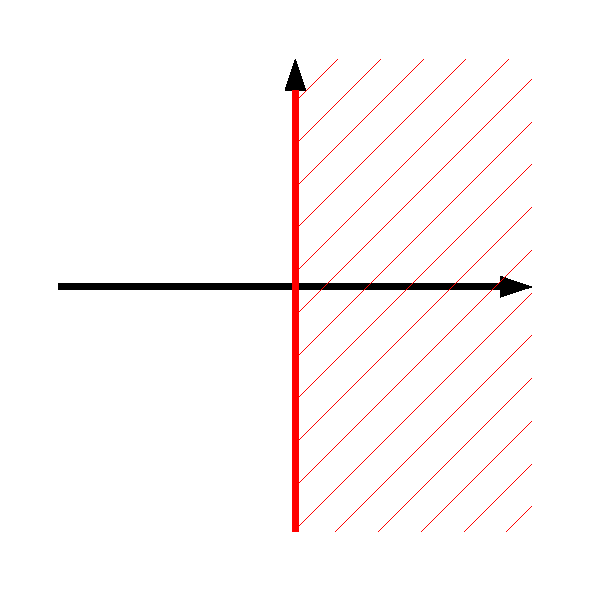
\includegraphics[width=4cm]{Content/01_theory/gebiet_1.pdf}\\

\end{minipage}
\begin{minipage}{4cm}
  	Gebiet:\\
  	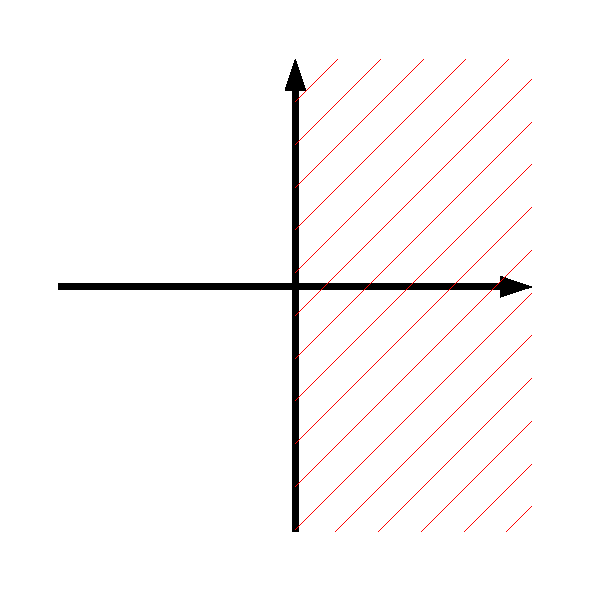
\includegraphics[width=4cm]{Content/01_theory/gebiet_2.pdf}\\
\end{minipage}

\textbf{Lösung einer PDGL:}\\
\begin{tabular}{ll}
Gegeben:& Gebiet $\Omega$, PDGL,Randwerte $\partial\Omega$\\
Lösung:& Funktion $u$: $\overset{\_}{\Omega}\rightarrow \mathbb{R}$, PDGL in $\Omega$ und Randwerte auf $\partial\Omega$\\
\end{tabular} \\
'gut gestellt' wen die Angaben die Lösung eindeutig bestimmen

\subsubsection{Klassifikation einer PDGL}
\begin{tabular}{lll}
Ordnung:& \multicolumn{2}{l}{Höchste vorkommende partielle Ableitung}\\
Typ:& Linear: & Linear in $u, x_1,...,x_n, \frac{\partial u}{\partial x_1},\ldots,\frac{\partial u}{\partial x_n}$\\
& Quasilinear: &  Linear in $\frac{\partial u}{\partial x_1},\ldots,\frac{\partial u}{\partial x_n}$\\
& Nichtlineare: & Alles andere
\end{tabular}


\subsection{Method of Characteristics}

\textbf{Important:} Characteristics \textbf{cannot} be used as initial conditions, otherwise the characteristic becomes the solution (instead of obtaining a surface, you get a curve).\\
\textbf{Important:} The characteristic must pass through the boundary only once.\\
Useful for Quasilinear PDEs of 1st order. If separation is possible, this (simpler) method should be used.

Initial condition:
\[
    a(x,y,u)\cdot\partFrac{u}{x}+b(x,y,u)\cdot\partFrac{u}{y}-c(x,y,u)=0
\]
Characteristic:
\[
    \frac{d}{dt} \begin{bmatrix} x(t) \\ y(t) \\ u(t) \end{bmatrix}
    = \begin{bmatrix} a(x,y,u) \\ b(x,y,u) \\ c(x,y,u) \end{bmatrix}
\]


\begin{tabular}{ll}
Region:& $\Omega\{\ldots|x>0, \text{all }y\}$\qquad Boundary condition: $u(0,y_0)=g(y_0)$\\
Vector notation:& $\begin{bmatrix}
    a(x,y,u)\\ b(x,y,u)\\ c(x,y,u)
    \end{bmatrix}
\underset{\overrightarrow{n}\text{: Normal to surface}}{\underbrace{\begin{bmatrix}
\partFrac{u}{x} & \partFrac{u}{y} & -1
\end{bmatrix}}}=0 $ \\[1cm]
Tangents:& $\overrightarrow{t}_x=\begin{bmatrix}1\\0\\ \partFrac{u}{x}\end{bmatrix}\qquad
			\overrightarrow{t}_y=\begin{bmatrix}0\\1\\ \partFrac{u}{y}\end{bmatrix}\qquad \overrightarrow{n} \bullet \overrightarrow{t_x} = 0 \qquad \overrightarrow{n} \bullet \overrightarrow{t_y} = 0 \qquad \overrightarrow{t_x} \bullet \overrightarrow{t_y} = \overrightarrow{n}$\\[1cm]

Solution approach: & For each initial point $\begin{bmatrix} 0\\y_0\\g(y_0)\end{bmatrix}$ find a characteristic, then solve for $x$, $y$.
\end{tabular}

\paragraph{Boundary Conditions}
A solution function $u(x,y)$ must be covered by characteristics.
The solution is now determined by the boundary values.

\begin{minipage}{10cm}
    For the depicted region $\Omega$, different cases are possible:
    \begin{enumerate}
        \item Boundary values on the \emph{left} and \emph{right} are given. A region in the middle is undetermined.
        \item Boundary values on the \emph{upper} and \emph{lower} boundaries are given. A part of the region is over-determined.
        \item Boundary values on the \emph{left} and \emph{lower} boundaries are given. The function is uniquely determined (but not necessarily differentiable everywhere).
    \end{enumerate}
    The solution is not determinable for all boundary values. \newline
    If two characteristics meet $\rightarrow$ Singularity
\end{minipage}
\hspace{0.5cm}
\begin{minipage}{8cm}
    \centering
    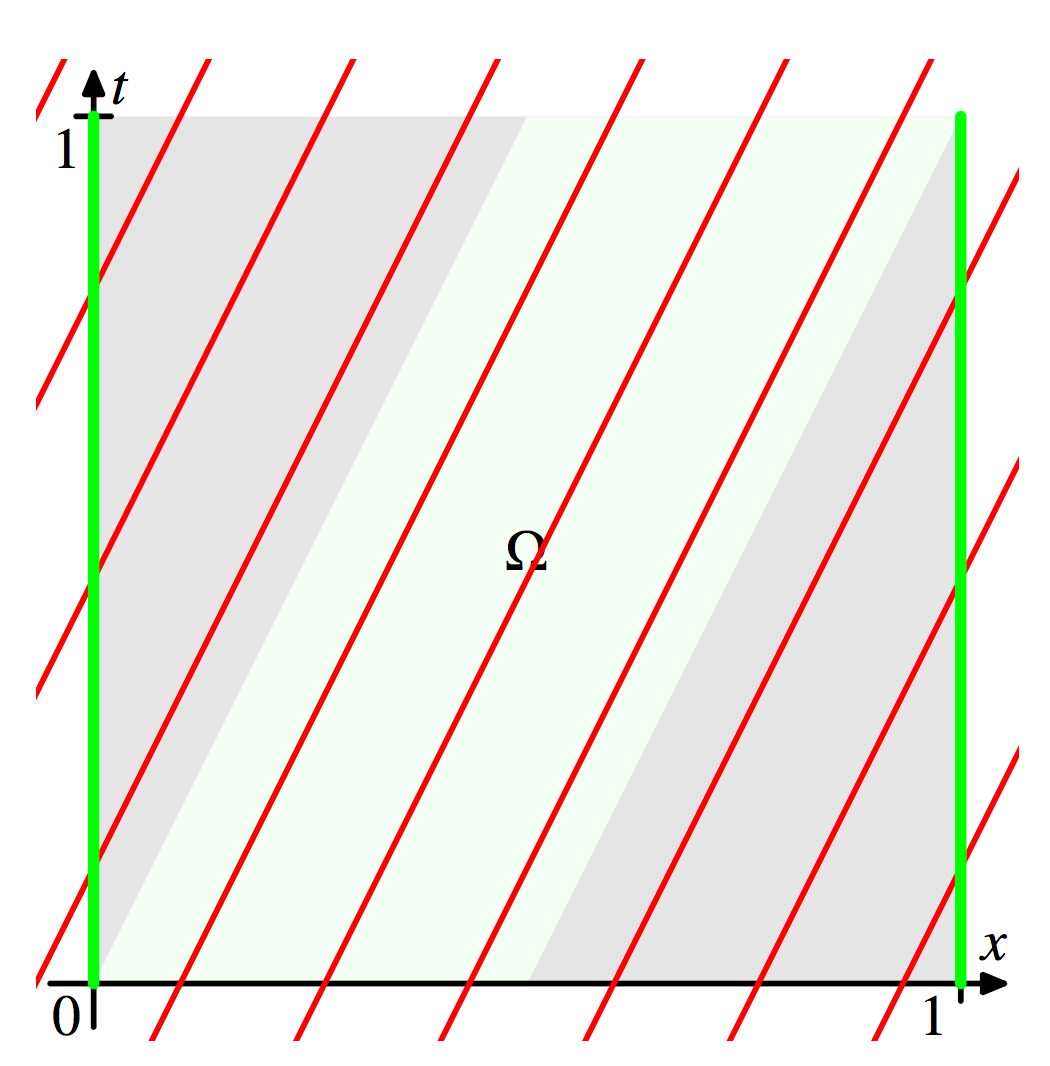
\includegraphics[width=6cm]{Content/01_theory/charakteristiken_randwerte.png}
\end{minipage}

\paragraph{Example:}~\\
\begin{enumerate}
	\item PDE with boundary conditions and domain: $\partFrac ux+2\partFrac uy=3$, \; $u(0,y)=g(y)=\sin(y) \Rightarrow u(0,y_0) = g(y_0) = \sin(y_0)$\\
	Terms in matrix form: $\begin{bmatrix}a\\b\\c\end{bmatrix}=\begin{bmatrix}1\\2\\3\end{bmatrix}$
	\item Calculate characteristics from PDE $\rightarrow$ ODE: 	$\frac {d}{dt}\begin{bmatrix}x(t)\\y(t)\\u(t)\end{bmatrix}=\begin{bmatrix}1\\2\\3\end{bmatrix}$
	\item Solve ODEs (for standard ODEs, see \ref{sec:dgls} on page \pageref{sec:dgls}.):
	$\begin{bmatrix}x\\y\\u\end{bmatrix}=\begin{bmatrix}1t+x_0\\2t+y_0\\3t+u_0\end{bmatrix}$
	\item Substitute initial conditions: $\begin{bmatrix}x\\y\\u\end{bmatrix}=\begin{bmatrix}1t+x_0\\2t+y_0\\3t+u_0\end{bmatrix}\Bigg|_{t=0}=
	\begin{bmatrix}x_0\\y_0\\u_0\end{bmatrix}=\begin{bmatrix}0\\y_0\\\sin(y_0)\end{bmatrix}$\\
	Solution of ODE is: $\begin{bmatrix}x\\y\\u\end{bmatrix}=\begin{bmatrix}1\\2\\3\end{bmatrix}\cdot t+ \begin{bmatrix}0\\y_0\\\sin(y_0)\end{bmatrix}$\\

	\item Eliminate all variables except $u,x,y$: $u=3x+\sin(y-2x)$
	\item Verification:
	Derive the result ($u=3x+\sin(y-2x)$) and substitute it into the original PDE $\partFrac ux+2\partFrac uy=3$ to check if it is satisfied.

\end{enumerate}


\subsection{Method Separation}
Choosing a suitable coordinate system is important.

\begin{enumerate}
\item \textbf{Approach} (Highest derivative decisive):
	\begin{itemize}
		\item For PDE 1st Order: $U(x,y)=X(x) + Y(y)$
		\item For PDE 2nd Order: $U(x,y)=X(x) \cdot Y(y)$
	\end{itemize}
\item \textbf{Substitution: } Substitute the approach into the PDE.
\item \textbf{Separation: } Each side of the PDE should only have one variable. The two resulting ordinary differential equations are coupled by a constant (fixing the variable). Choice of constant: If oscillation is expected, $-k^2$, otherwise $k$, unless you know better ;-).
\item \textbf{Solving the ODEs: } Obtain a family of solutions
\item \textbf{Constructing the General Solution: } (Linear combination of solutions), adhere to boundary conditions!
\end{enumerate}

\begin{minipage}{0.49\textwidth}
\textbf{Example 1: } PDE: $\frac1x\partFrac{u}{x}+\frac1y\partFrac{u}{y}=\frac{1}{y^2}$
\begin{enumerate}
	\item Approach:\\[0.4cm]
	$u(x,y)=X(x) + Y(y)$ (1st Order)
	\item Substitution:\\[0.4cm]
	$\partFrac{u}{x}=X'(x)$\qquad $\partFrac{u}{y}=Y'(y)$ \quad $\Rightarrow$ \quad $\frac{X'(x)}{x}+\frac{Y'(y)}{y}=\frac{1}{y^2}$
	\item Separation:\\[0.4cm]
	$\frac{X'(x)}{x}=k=\frac{1}{y^2}-\frac{Y'(y)}{y}$
	\item Solving ODEs:\\[0.4cm]
	$X'(x)=k\cdot x \quad\Rightarrow\quad X(x)=\frac12 kx^2+C_x$\\
	$Y'(y)=\frac1y-ky \quad\Rightarrow\quad Y(y)=\ln(y)-\frac12 ky^2+C_y$
	\item Linear Combination:\\[0.4cm]
	$u(x,y)=\frac12 kx^2 - \frac12 ky^2+ln(y)+C$
\end{enumerate}

\textbf{Example 2: } PDE: $x^2\partFrac{^2u}{x^2}+x\partFrac{u}{x}+y^2\partFrac{^2u}{y^2}+y\partFrac{u}{y}=0$\\
Boundary conditions: $\Omega=[1,2]\times[1,2]$ \qquad $u=0$ on $\partial\Omega$
\begin{enumerate}
	\item Approach:\\[0.4cm]
	$u(x,y)=X(x) \cdot Y(y)$ (2nd Order)
	\item Substitution:\\[0.4cm]
	$x^2X''(x)Y(y)+xX'(x)Y(y)+y^2X(x)Y''(y)+yX(x)Y'(y)=0$
	\item Separation: Division by $X(x)Y(y)$\\[0.4cm]
	$\frac{x^2X''(x)}{X(x)}+\frac{xX'(x)}{X(x)}+\frac{y^2Y''(y)}{Y(y)}+\frac{yY'(y)}{Y(y)}=0\quad\Rightarrow\quad \frac{x^2X''(x)}{X(x)}+\frac{xX'(x)}{X(x)}=k=-\frac{y^2Y''(y)}{Y(y)}-\frac{yY'(y)}{Y(y)}$
	\item Solving ODEs:\\[0.4cm]
	$\frac{x^2X''(x)}{X(x)}+\frac{xX'(x)}{X(x)}=k\quad\Rightarrow\quad x^2X''(x)+xX'(x)-kX(x)=0$\qquad with $X(1)=X(2)=0$\\
	$\frac{y^2Y''(y)}{Y(y)}-\frac{yY'(y)}{Y(y)}=-k\quad\Rightarrow\quad y^2Y''(y)+yY'(y)+kY(y)=0$\qquad with $Y(1)=Y(2)=0$\\[0.4cm]
	Solution of ODEs not done here.
\end{enumerate}
\end{minipage}
\hfill
\begin{minipage}{0.49\textwidth}
\textbf{Example 3: }PDE: $\partFrac{^2u}{t^2}=\partFrac{^2u}{x^2}$ \quad $u(t=0,x)=0$\\
Boundary conditions: $x=[0,\pi]$ \\
\qquad\qquad $\partFrac{u}{t}(t=0,x)=\sin^3(x)=\frac34\sin(x)-\frac14\sin(3x)$
\begin{enumerate}
	\item Approach:\\[0.4cm]
	$u(t,x)=T(t) \cdot X(x) $ (2nd Order)
	\item Substitution:\\[0.4cm]
	$T''(t)\cdot X(x) = X''(x)\cdot T(t)$
	\item Separation:\\[0.4cm]
	$\frac{X''(x)}{X(x)}= -\mu^2=\frac{T''(t)}{T(t)}$
	\item Solving ODEs:\\[0.4cm]
		$X(x)=\sin(\mu x) \qquad T(t)=\sin(\mu t)$\\
		$X(x)=\cos(\mu x) \qquad T(t)=\cos(\mu t)$
	\item Linear Combination:\\[0.4cm]
		The boundary conditions $x=0$ and $x=\pi$ can only be satisfied with $\sin(\mu x) $ and positive, integer $\mu$. $cos(nx)$ terms are eliminated.\\[0.4cm]
		$u(t,x)=\sum\limits_{n=1}^{\infty}{a_n\sin(nx)\sin(nt)} + \sum\limits_{n=1}^{\infty}{b_n\sin(nx)\cos(nt)}$\\[0.4cm]
		The coefficients $a_n$ and $b_n$ must be determined using the initial conditions at time $t=0$:\\[0.4cm]
		$u(0,x)=\sum\limits_{n=1}^{\infty}{b_n\sin(nx)}=0 \quad\Rightarrow\quad b_n=0$\\[0.2cm]
		$\partFrac{u}{t}(\pi,x)=\sum\limits_{n=1}^{\infty}{a_nn\sin(nx)}=\sin^3(x)=\frac34\sin(x)-\frac14\sin(3x) \quad\Rightarrow\quad a_1=\frac34 \quad a_3=-\frac{1}{12}\quad a_k=0$ for $k\neq 1,3$\\[0.4cm]
		$u(t,x)=\frac34\sin(x)\sin(t)-\frac1{12}\sin(3x)\sin(3t)$
\end{enumerate}
\end{minipage}


\subsection{Hamilton-Jacobi Theorie}
Die Hamilton-Jacobi Theorie geht von einer Gesamtenergie $H(x_i,p_i)$ in Abhängigkeit von Ort
und Impuls aus.
Dazu muss eine Funktion $S(x_i,t)$ gefunden werden, für welche
\begin{align*}
    \frac{\partial S}{\partial t} = H\left(x_i,p_i\right) = H\left(x_i,\frac{\partial S}{\partial x_i}\right)
    && \text{mit} \quad
    p_i = \frac{\partial S}{\partial x_i}
\end{align*}
Diese kann meist durch Integration gelöst werden.
Dabei werden die Integrationskonstanten $P_i$ eingeführt.
Die \emph{Bahnparameter} $Q_i$ sind
\[
    Q_i = \frac{\partial S}{\partial P_i}
\]
und die Bahnkurve hat die Form
\[
    x_i(t,Q_i,P_i)
\]

\begin{landscape}

\begin{minipage}{7cm}
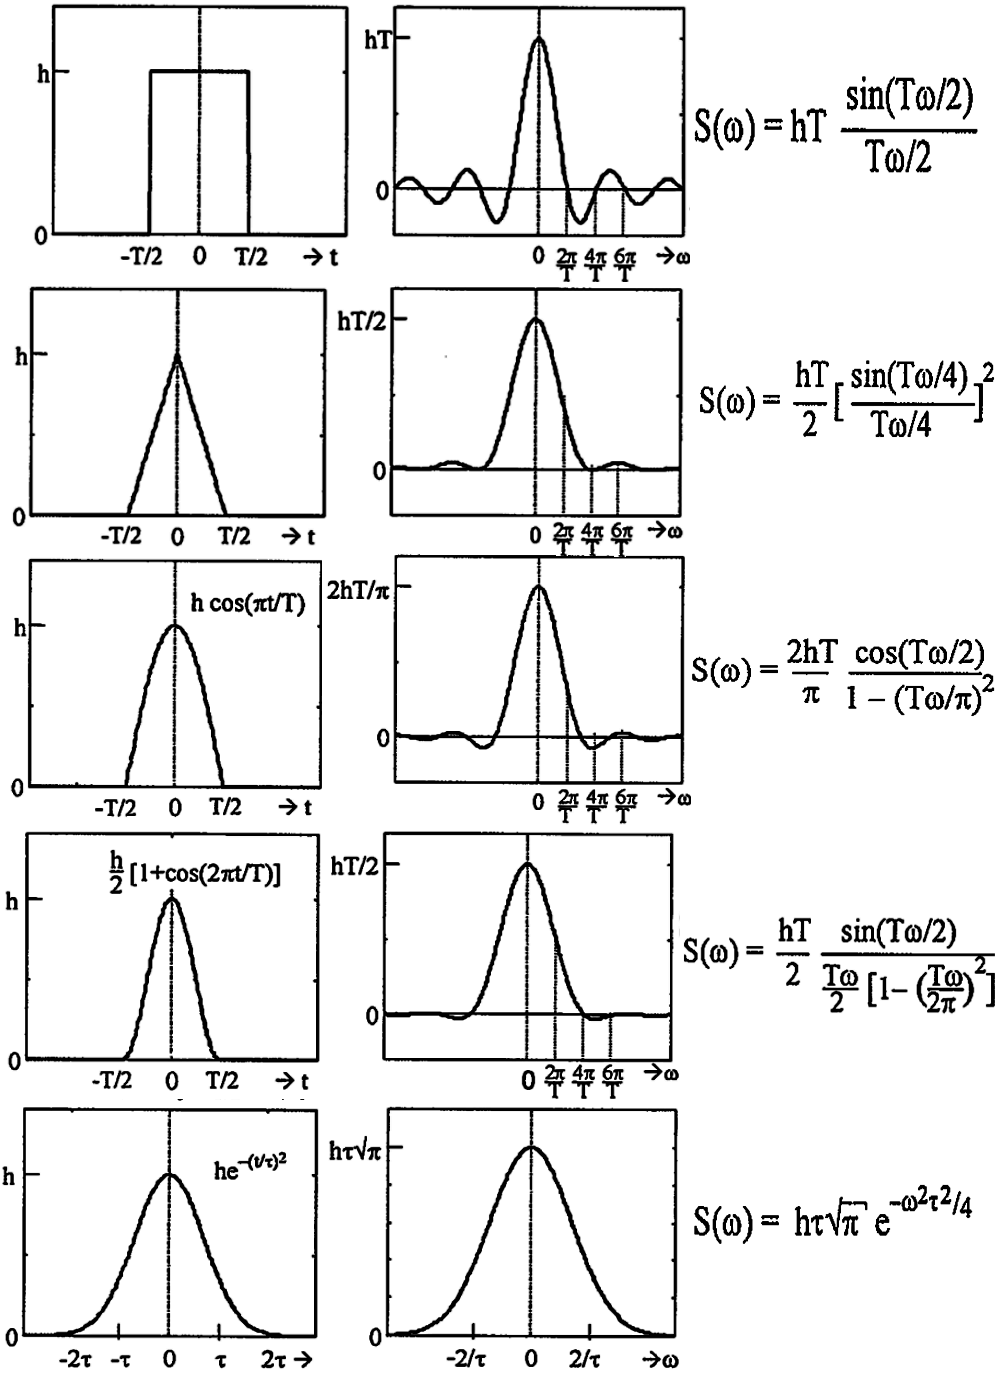
\includegraphics[width=\textwidth,trim= 0cm 0cm 0cm 0cm]{bilder/Transformationen/Fourier-Trafo.png}

\end{minipage}
\begin{minipage}{8.25cm}
	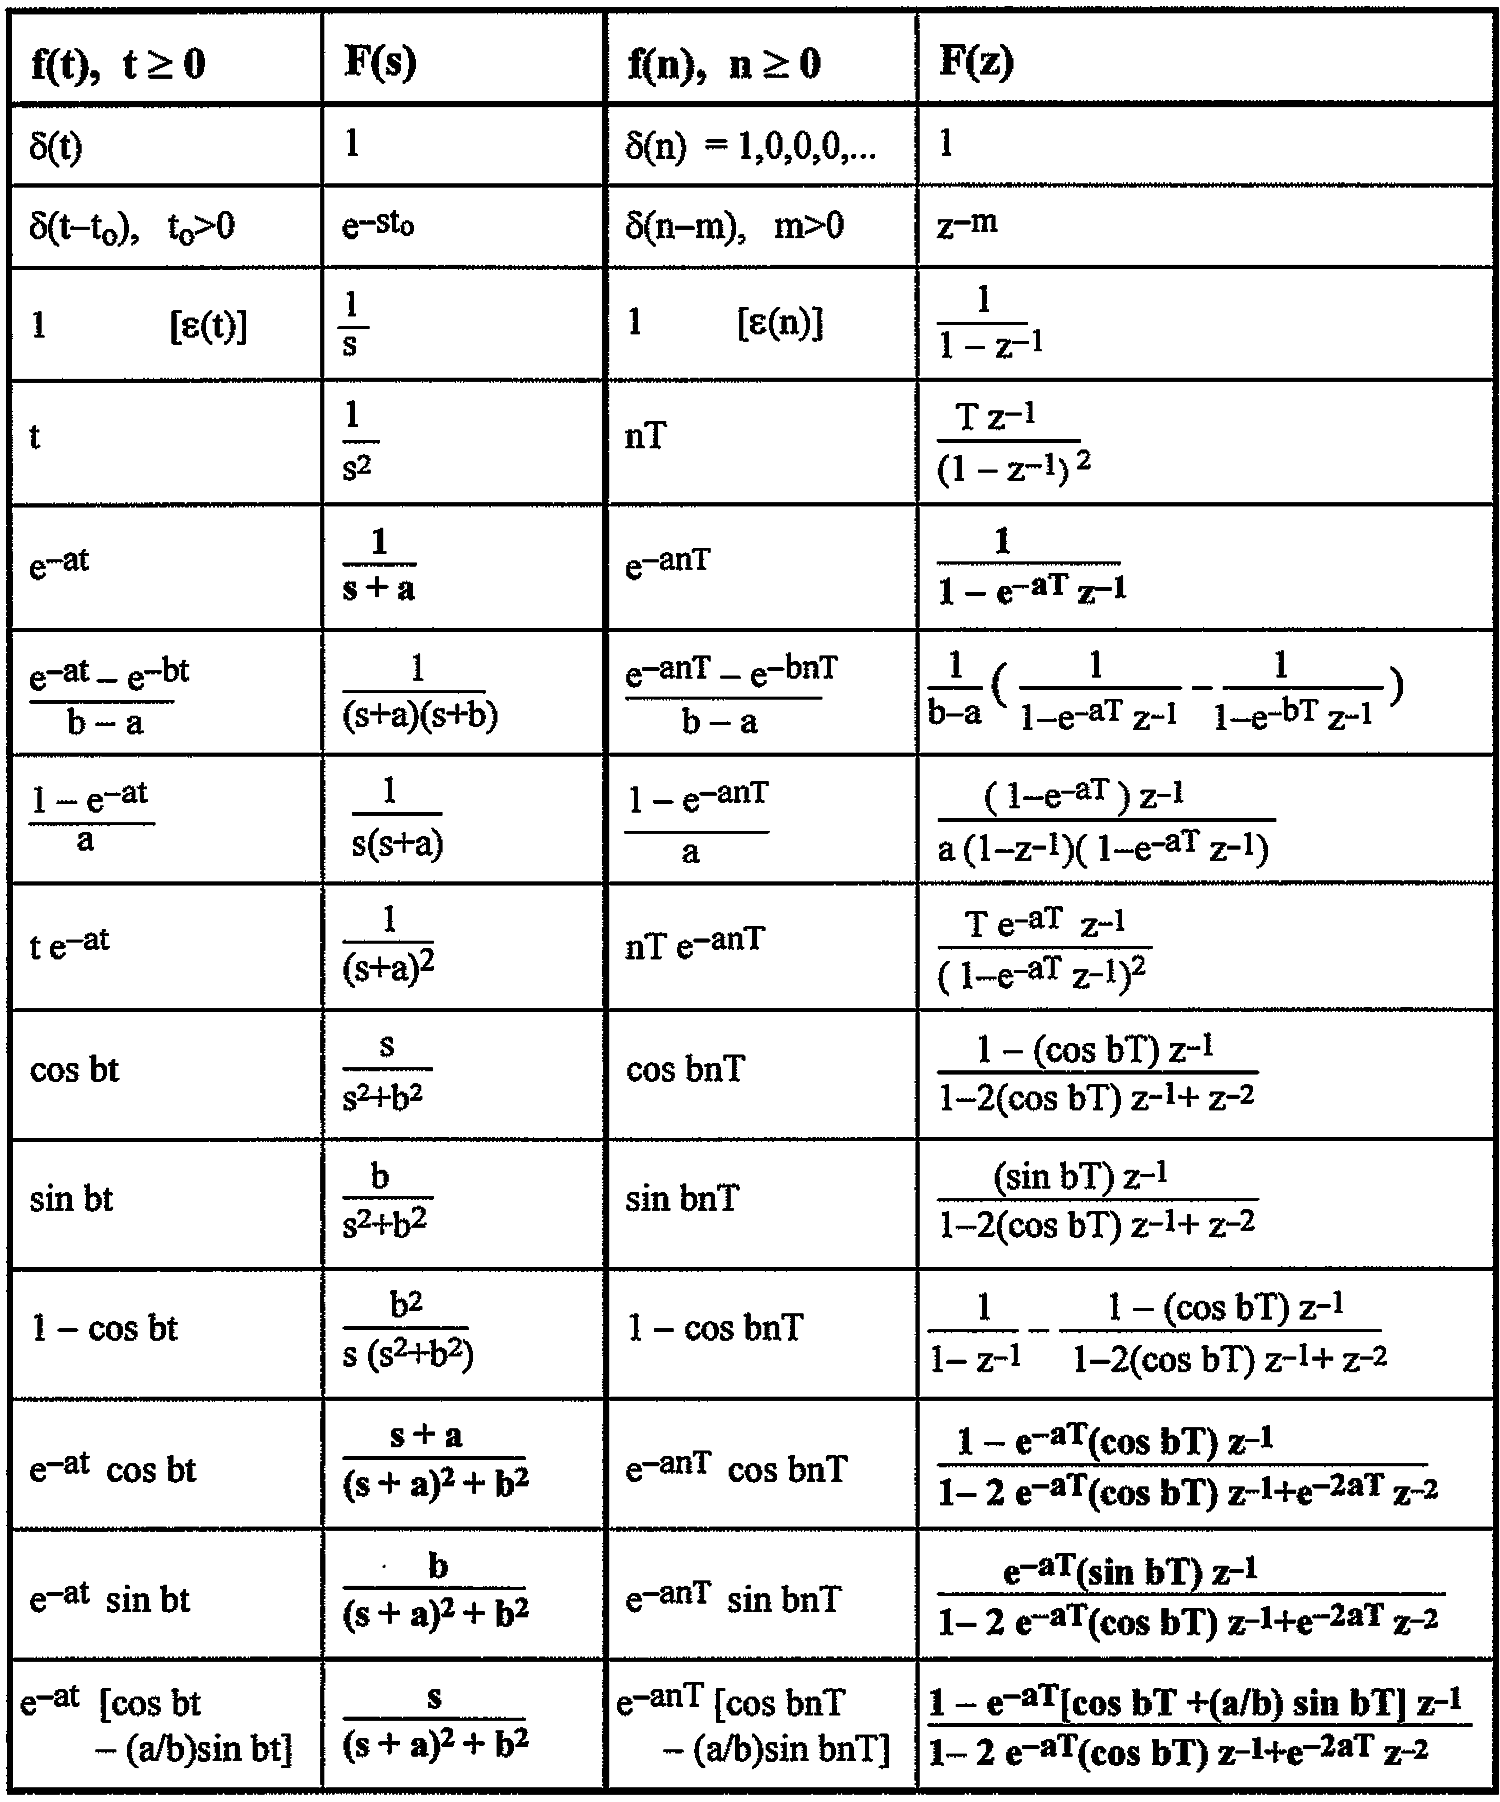
\includegraphics[width=\textwidth,trim= 0cm 0.3cm 0cm 0.45cm]{bilder/Transformationen/Z-Lexikon.png}
	\end{minipage}
	\begin{minipage}{10cm}
	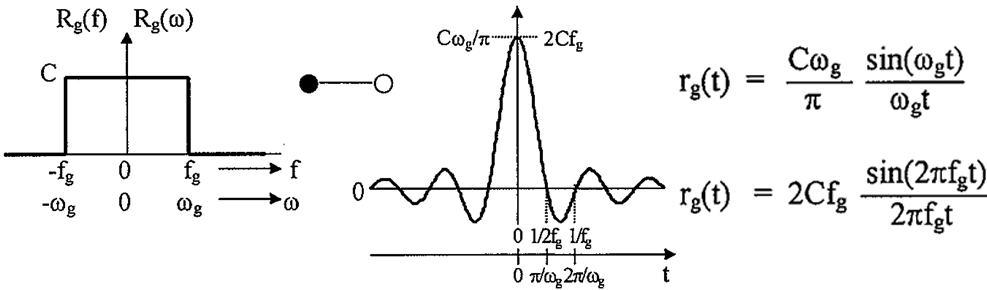
\includegraphics[width=\textwidth,trim= 0cm 0cm 0cm 0cm]{bilder/Transformationen/Rechteck-Sinc.png}
	\textbf{Matrizeninversion}\\
	$A^{-1} = \begin{pmatrix}
	a & b \\ c & d \\
	\end{pmatrix}^{-1} =
	\frac{1}{\det(A)} \begin{pmatrix}
	d & -b \\ -c & a \\
	\end{pmatrix}  =
	\frac{1}{ad-bc} \begin{pmatrix}
	d & -b \\ -c & a \\
	\end{pmatrix}\quad$\\
	$A^{-1} = \begin{pmatrix}
	a & b & c\\ d & e & f \\ g & h & i \\
	\end{pmatrix}^{-1} =
	\frac{1}{\det(A)} \begin{pmatrix}
	ei - fh & ch - bi & bf - ce \\
	fg - di & ai - cg & cd - af \\
	dh - eg & bg - ah & ae - bd
	\end{pmatrix}$\\
	\begin{minipage}{4cm}
		\textbf{Trigonometrie} \\
		$e^{j\varphi}=\cos(\varphi)+ j \cdot \sin(\varphi) $
		$e^{-j\varphi}=\cos(\varphi)- j \cdot \sin(\varphi) $
		$\cos(x) = \frac{e^{jx} + e^{-jx}}{2}$\\
		$\sin(x) = \frac{e^{jx} - e^{-jx}}{2j}$\\
		$\cos^2(x) = \frac12 + \frac{\cos(2x)}{2}$\\
		$\sin^2(x) = \frac12 - \frac{\cos(2x)}{2}$\\
		$\sin(2x)=2\sin(x)\cdot\cos(x)$\\
		$\sin^2(x)+\cos^2(x)=1$
	\end{minipage}
	\begin{minipage}{5cm}
		\textbf{Determinanten} \\
		\footnotesize
		$\det \begin{pmatrix} a & b \\ c & d\\ \end{pmatrix} =
		a d - b c \quad$\\
		$\det \begin{pmatrix} 
		a & b & c \\
		d & e & f \\
		g & h & i  \end{pmatrix}
		= a e i + b f g + c g h \\
		\text{\hspace{2.5cm}} -c e g - f h a - i b d$		\normalsize
	\end{minipage}
\end{minipage}

%\section{Fourier Transformation}
\begin{minipage}{0.85\linewidth}
%\subsubsection{Eigenschaften von Fourier- und Z-Transformation}
\footnotesize 
\renewcommand{\arraystretch}{1.1}
\begin{tabular}{|p{4.3cm}||p{1.8cm}|p{1.8cm}||p{2.2cm}|p{2.4cm}||p{1.9cm}|p{2.6cm}|}
\hline
\textbf{Bezeichnung}
  & \multicolumn{2}{|c||}{\textbf{Zeitbereich}}
  & \multicolumn{2}{|c||}{\textbf{Kontinuierlicher Frequenzbereich}}
  & \multicolumn{2}{|c|}{\textbf{Diskreter Frequenzbereich}} \\
  & \textbf{kontinuierlich}
  & \textbf{diskret}
  & \textbf{Fourier-Integral} 
  & \textbf{Laplace}
  & \textbf{Diskrete FT} 
  & \textbf{Z-Transformation} \\
\hline
\hline
  Linearität 
  & $\alpha\cdot f(t) + \beta\cdot g(t)$
  & $\alpha\cdot f(n) + \beta\cdot g(n)$
  & $\alpha\cdot F(\omega) + \beta\cdot G(\omega)$
  & $\alpha\cdot F(s) + \beta\cdot G(s)$
  & $\alpha\cdot F(n) + \beta\cdot G(n)$
  & $\alpha\cdot F(z) + \beta\cdot G(z)$\\
\hline
  "Ahnlichkeit / Zeitskalierung bzw. Spiegelung an Y-Achse
  &	$f(\alpha t)$ 
  & $f(-n)$
  & $\frac{1}{|\alpha|}F \left (\frac{\omega}{\alpha} \right)$
  & $\frac{1}{\alpha}F \left (\frac{s}{\alpha} \right )$ 
  & $F(-n)$
  & $F(z^{-1})$\\
%\hline
  %D�mpfung
  %& -
  %& $e^{dn} f(n)$
  %& -
  %& - 
  %& -
  %& $F(z e^{d})$ \\
\hline
  Verschiebung im Zeitbereich 
  & $f(t\pm t_0)$ 
  & $f(n \pm n_0)$
  & $e^{\pm j\omega t_0} F(\omega)$
  & $F(s)e^{\pm t_0 s}$ 
  & $e^{\pm j\frac{n}{N}2 \pi n_0} F(n)$
  & $z^{\pm n_0} F(z)$\\
\hline
  Verschiebung im Frequenzbereich 
  & $f(t)e^{\mp\alpha t}$ 
  & $f(n) e^{\mp j \frac{n}{N} 2 \pi n_0}$
  & $F(\omega\pm \alpha)$
  & $F(s\pm\alpha)$ 
  & $F(n \pm n_0)$
  & $F(z \pm n_0)$\\
\hline
  Faltung im Zeitbereich 
  &	$f(t) \ast g(t)$
  & $f(n) \ast g(n)$
  & $F(\omega) \cdot G(\omega)$
  & $F(s) \cdot G(s)$
  & $F(n) \cdot G(n)$ 
  & $F(z) \cdot G(z)$ \\
\hline
  Faltung im Frequenzbereich 
  &	$f(t) \cdot g(t)$
  & $f(n) \cdot g(n)$
  & $\frac{1}{2\pi} F(\omega) \ast G(\omega)$
  & $\frac{1}{2\pi} F(s) \ast G(s)$ 
  & $\frac{1}{N} F(n) \ast G(n)$
  & $\frac{1}{N} F(z) \ast G(z)$\\
\hline
  Ableitungen im Zeitbereich bzw. Differenzenbildung 
  & $\frac{\partial^n f(t)}{\partial t^n}$ 
  & $\Delta^k f(n)$
  & $(j\omega)^n F(\omega)$
  & $s^nF(s)-s^{n-1}f(0+)-s^{n-2}\frac{\partial f(0+)}{\partial t}-\ldots
 			-s^0\frac{\partial^{n-1} f(0+)}{\partial t^{n-1}}$
  & 
  & $(1-z^{-1})^k F(z)$ \\
\hline
  Ableitung im Frequenzbereich
  & $(-t)^k\cdot f(t)$ 
  & $n f(n)$ 
  & $j^k \frac{-\partial^k F(\omega)}{\partial \omega^k}$
  & $\frac{\partial^k F(s)}{\partial s^k}$
  & 
  & $-z \frac{\partial F(z)}{\partial z}$ \\
\hline 			
  Integration bzw. Summierung
  & $\int\limits_{-\infty}^t f(\tau)d\tau$ 
  & $\sum\limits_{n=0}^{k} f(n)$
  & $\frac{F(\omega)}{j\omega}+F(0)\pi\delta(\omega)$
  & $\frac{F(s)}{s}$
  & 
  & $\frac{1}{1-z^{-1}} F(z)$ \\
\hline
  Anfangswert 
  & $\lim\limits_{t\rightarrow 0} f(t)$ 
  & $f(0)$
  & 
  & $\lim\limits_{s\rightarrow \infty} sF(s)$ 
  & 
  & $\lim\limits_{z \rightarrow \infty} F(z)$ \\
\hline
  Endwert
  &	$\lim\limits_{t\rightarrow \infty} f(t)$
  & $\lim\limits_{n\rightarrow \infty} f(n)$
  & 
  & $\lim\limits_{s\rightarrow 0} sF(s)$
  & 
  & $\lim\limits_{z \rightarrow 1} (1-z^{-1}) F(z))$\\
%\hline
  %Stabilit�t
  %& -
  %& -
  %& -
  %& Pole in LHE
  %& 
  %& Pole innerhalb Einheitskreis \\
%\hline
  %Kausalit�t
  %& -
  %& -
  %& A- \& Kausal
  %& Nur Kausal
  %& 
  %& $\lim\limits_{z \rightarrow \infty} z^{-1} F(z) = 0$ \\
\hline
\hline
  Spezial
  & \multicolumn{3}{l||}{
      Bessel-Theorem \qquad
      $\int\limits_{-\infty}^{\infty}f(t)g^{\ast}(t)dt =
         \frac{1}{2\pi}
         \int\limits_{-\infty}^{\infty}F(\omega)G^{\ast}(\omega)d\omega$}
  & \multicolumn{3}{|l|}{
      Parseval-Theorem \qquad
      $W = \int\limits_{-\infty}^{\infty}|f(t)|^2 dt = \frac{1}{2\pi}
      \int\limits_{-\infty}^{\infty}|F(\omega)|^2 d\omega$
    }\\
\hline

\end{tabular}
\end{minipage}
\begin{minipage}{0.2\linewidth}
\textbf{Quadratische Gleichung:}\\
$a\cdot x^2+b\cdot x +c=0$\\

$x_{1,2}=\frac{-b\pm \sqrt{b^2-4ac}}{2a}$\\

\textbf{Fouriertransformation:}\\

$\delta(t)\FT 1$\\
$1\FT 2\pi \delta(\omega)$\\
$\sigma(t)\FT \frac{1}{j\omega}+\pi\delta(\omega)$\\
$\text{sgn}(t)\FT \frac{2}{j\omega}$\\
$e^{\pm j \omega_0 t} \FT 2\pi \delta(\omega \mp \omega_0)$\\
$\sin(\omega_0t)\FT j\pi(\delta(\omega +\omega_0)-\newline\text{\hspace{2.7cm}}\delta(\omega -\omega_0))$\\
$\cos(\omega_0t)\FT \pi(\delta(\omega +\omega_0)+\newline\text{\hspace{2.6cm}}\delta(\omega -\omega_0))$\\
\end{minipage}


%% We don't need this and it does not fit onto the page. The trigonometric relationships are already on this page under ''Trigonometrie'', and the z-transforms are in the z-transform table. 
%% In my opinion the z-transform table should also be updated, because you can barely read it when it's included as a picture and scaled. 
 
% \begin{minipage}{\linewidth}
% \vspace*{-1cm}
% $e^{j\omega}=\cos(\omega) + j \cdot \sin(\omega)$
% \quad
% $\sin(\omega)=\dfrac{e^{j\omega} - e^{-j\omega}}{2j}$
% \quad
% $\cos(\omega)=\dfrac{e^{j\omega} + e^{-j\omega}}{2}$
% \quad
% $1\pm e^{-j\omega T}= (e^{j\frac{\omega}{2} T}\pm e^{-j\frac{\omega}{2} T})\cdot e^{-j\frac{\omega}{2} T}$
% \quad
% $a^n \FT \frac{1}{1-az^-1}$
% \quad
% $a^{|n|} \FT \frac{1-a^2}{(1-az^-1)(1-az)}$
% \quad
% \vspace*{-2cm}
% \end{minipage}


\end{landscape}

\subsection{PDE 2nd Order}
Linear partial differential equations of second order have the form:
$\boxed{\sum\limits_{i,j=1}^{n}{a_{ij}\partial_i\partial_j u}+\sum\limits_{i=1}^{n}{b_i\partial_i u}+cu=f}$

\subsubsection{Classification}
Classification only for PDEs of second order!

\begin{minipage}{9cm}
  Eigenvalue calculation: (e.g., for $ \partial^2_xu+2\partial_x\partial_yu+\partial^2_yu=0 $)
  \begin{enumerate}
    \item Form a symmetric matrix and subtract $\lambda$ on the diagonal. For example: $A = \begin{pmatrix}
      \partial_x^2 & \partial_x \partial_y \\
      \partial_y \partial_x  & \partial_y^2
    \end{pmatrix}$\\
    In diagonal matrices, the eigenvalues correspond to the diagonal entries.
    \item Set determinant equal to 0: $\det(\mathbf{A}-\lambda \mathbf{I}) = 0\quad\Rightarrow\quad \lambda_i$
    \item Solve the equation
  \end{enumerate}
\end{minipage}
\hfill
\begin{minipage}{9cm}
  Alternatively (if, for example, a very complicated PDE needs to be classified), the signs of the eigenvalues can also be determined via trace and determinant:
  \begin{enumerate}
    \item See left (Eigenvalue calculation): Form matrix $A$
    \item Calculate determinant and try to read from the table:
     $\det A = a_{11}a_{22} - a_{12}a_{21} = \lambda_1 \lambda_2$
    \item Calculate trace and try to read from the table:
      $\tr(A) = a_{11} + a_{22} = \lambda_1 + \lambda_2$
  \end{enumerate}
\end{minipage}

\begin{center}
\begin{tabular}{|l||l|l|l|l|l|}
\hline
\multirow{2}{*}{Class}&\multicolumn{3}{|c|}{Number of Eigenvalues} & det(A)&\multirow{2}{*}{Example}\\
& Positive & Negative & Zero(=0) & for n=2 &\\
\hline
Hyperbolic& n-1 & 1 & 0 & det < 0 & Wave Equation: $\frac{\partial^2 u}{\partial t^2} = \Delta u$ \\
\hline
Parabolic& n-1 & 0 & 1 & det = 0 & Heat Equation: $\frac{\partial u}{\partial t} = \Delta u$  \\
\hline
Elliptic&	n & 0 & 0 & det > 0 & Potential: $\Delta u = f$ \\
\hline
Ultrahyperbolic & >1 & >1 & 0 & - & -\\
\hline
\end{tabular}
\end{center}


\subsection{Elliptische PDGL}
$\Delta u=f\qquad \omega=\{(x,y)|y\geq 0\},\quad u(x,y)=ay$

\textbf{Satz:} Wenn $\Omega$ beschränkt und zusammenhängend, dann ist die Lösung u immer eindeutig.\\

\textbf{Beweis:} Annahme: $u=u_1-u_2$\\
Einsetzen: $\Delta u_1 - \Delta u_2=f-f=0$\\
$\left.(u_1-u_2)\right|_{\partial \omega}=g-g=0$\\
$\Delta u=0 \qquad \left.u\right|_{\partial\Omega}=0$\\
Falls $u=0$ eine Lösung, dann gibt es nur eine Lösung.

\subsubsection{Maximumprinzip} 

Wenn gilt $\Delta u=0$, so ist $u$ \emph{harmonisch}, und dann befinden 
sich die Extrema (Maxima und Minima der Funktion) auf dem Rand $\partial\Omega$.

\subsubsection{Beispiel (Übungslösungen)}
Eine elliptische PDGL wie $\Delta u = c$ hat mit der vorgegebenen
Dirichlet-Randwerten nur eine Lösung. Zur Erinnerung: Der Grund war das
Maximum-Prinzip. Gäbe es nämlich eine zweite Lösung $\bar v(r,\phi)$ mit
gleichen Randwerten, wäre $v - \bar v$ eine Lösung der Gleichung $\Delta (v -
\bar v) = 0$ also harmonische Funktion. Die Randwerte von $v - \bar v$ sind 0. Da eine
harmonische Funktion das Maximum auf dem Rand annimmt ist $v - \bar v = 0$ die
Lösung ist also eindeutig.

\newpage
\subsubsection{Greensche Funktion} 

Eine elliptische PDGL wird mittels Inversion von $\Delta$ gelöst. Dieser Umkehr geschieht mittels Greenscher Funktion, welche die Umkehrfunktion $\Delta$ ist\qquad $\Delta$: Laplace-Operator.

$u(x)=\int\limits_\Omega{\sigma(x,\xi)f(\xi)d\xi}+\int\limits_\Omega{h(x,\xi)f(\xi)d\xi}\qquad \sigma(x,\xi)=
\begin{cases}
	\frac 12|x-\xi| & n=1\\ 
	\frac 1{2\pi}\log|x-\xi| & n=2\\
	-\frac 1{4\pi}\frac{1}{|x-\xi|} & n=3\\
	\frac {1}{(2-n)\mu(S^{n-1})}|x-\xi|^{2-n} & n\geq 3\\
\end{cases}$\\


Greensche Funktion: $G(x,\xi)=\sigma(x,\xi)+h(x,\xi)$

Satz: Ist $\Omega$ ein Gebiet, auf dem das Dirichlet Problem eindeutig lösbar ist, dann gibt es eine Funktion $G(x,\xi)$, welche als Funktion von x die Gleichung

$\Delta G(x,\xi)=\delta(x-\xi)$

löst mit homogenen Randbedingungen.
Lösung: $u(x)=\int\limits_{\Omega}^{}{G(x,\xi)f(\xi)d\xi}+\int\limits_{\partial\Omega}g(\xi)\cdot\grad{\xi}G(x,\xi)d\eta\qquad \eta:\text{ Normale von }\partial G$

\subsubsection{Mittelwerteigenschaft harmonischer Funktionen}

$\Delta h=0$\qquad Mittelwerteigenschaft:\qquad $h(x)=
\begin{cases}
	\frac{h(x+\delta)+h(x-\delta)}{2}& n=1 \\ 
	\frac 1{2\pi r} \int\limits_{S_r^1}{h(x+\xi)d\xi} & n=2\\
	\frac 1{4\pi r^2} \int\limits_{S_r^2}{h(x+\xi)d\xi} & n=3\\
\end{cases}$
%\subsection{Parabolische PDGL}
\todo{Beschreibung}
\subsection{Hyperbolische PDGL}
\begin{minipage}{14cm}
	PDGL: $\partFrac{^2u}{t^2}-a^2\partFrac{^2 u}{x^2}=0\qquad \Omega=\left\{(x,t)|t>0\right\}\qquad u_0=u(x_0,0)$\\
	
	Trick: $(\partial_t +a\partial_x)(\partial_t-a\partial_x)u=(\partial_t^2-a^2\partial_x^2)u=0$\qquad(für konstante Geschwindigkeit $a$)\\
	
	Zwei mögliche Lösungen: $\underset{\text{\cfbox{red}{Nach rechts laufende Welle}}}{\underbrace{(\partial_t +a\partial_x)u=0}}\qquad \underset{\text{\cfbox{black}{Nach links laufende Welle}}}{\underbrace{(\partial_t-a\partial_x)u=0}}$\\
	
	Lösung mittels Charakteristiken: $\partFrac{}{s}
	\begin{Bmatrix}
		x(s)\\
		t(s)\\
		u(s)
	\end{Bmatrix}=
	\begin{Bmatrix}
		\pm a\\
		1\\
		0
	\end{Bmatrix}
	\begin{array}{ll}
		\Rightarrow&x=\pm as +x_0\\
		\Rightarrow&t= s +t_0=s\qquad (t_0=0)\\
		\Rightarrow&u=u_0\\
	\end{array}
	$\\
	
	$x=\pm at+x_0\quad\Rightarrow\quad x_0=x\mp at\quad\Rightarrow\quad u(x,t)=u_0(x\mp at)$\\
	
	Allgemeine Lösung aus Linearkombination: $\boxed{u(x,t)=u_+(x+at)+u_-(x-at)}$\\
	
	$\Rightarrow$ Es werden \textbf{zwei} Anfangsbedingungen benötigt um $u_+$ \textbf{und} $u_-$ zu bestimmen.\\
	
	z.B.: $u(x,0)=u_0(x)\qquad \partFrac{u}{t}(x,0)=g_0(x)$
	\end{minipage}
	\hfill
	\begin{minipage}{5cm}
	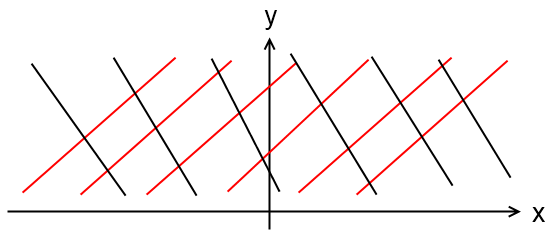
\includegraphics[width=5cm]{Content/01_theory/linksRechts}
	\end{minipage}
\subsubsection{Streifen/Charakteristiken}
	PDGL: $a\partial_x^2u+2b\partial_x\partial_yu+c\partial_y^2u+d\partial_xu+e\partial_yu+fu=g$ Symbolmatrix: $ 
		\begin{bmatrix}
			a & b\\
			b & c
		\end{bmatrix}$
	
	Entlang der Kurve $t\mapsto(x(t),y(t))$ sind die Anfangswerte / partiellen Ableitungen
	$
	\left.
	\begin{aligned}
	u(x(t),y(t))&=u(t)\\
	\partial_xu(x(t),y(t))&=p(t)\\
	\partial_yu(x(t),y(t))&=q(t)
	\end{aligned}
	\qquad
	\right\}
	\label{charanfangs}
	$
	
	Charakteristiken erfüllen DGL:
    \[
        a\dot y(t)^2-2b\dot x(t)\dot y(t)+c\dot x(t)^2=0
    \]
	
	Charakteristischer Streifen erfüllt zusätzlich: $a\dot p(t)\dot y(t)-h\dot x(t)\dot y(t)+c\dot x(t)\dot q(t)=0$


